\documentclass[12pt]{article}
\usepackage[utf8]{inputenc}
\usepackage{indentfirst}
\usepackage{graphicx}
\usepackage{hyperref}
\hypersetup{
    colorlinks,
    citecolor=black,
    filecolor=black,
    linkcolor=red,
    urlcolor=blue,
}
\usepackage{subcaption}

\title{Rapport de Stage \\ CR System}
\author{Cinquanta Octave \\ Étudiant à CY Tech}
\date{Février - Août 2026}

\begin{document}

\begin{figure}
    \captionsetup[subfigure]{labelformat=empty}
    \centering
    \subcaptionbox{}{%
        
\includegraphics[width=0.30\textwidth]{CR.png}}\hfill
    \subcaptionbox{}{%
        
\includegraphics[width=0.30\textwidth]{CY_Tech.svg.png}}
\end{figure}

\maketitle

\section{Sommaire}

Ce rapport présente un stage de six mois réalisé chez CR System, autour d’un objectif commun : transformer des tâches techniques récurrentes en outils fiables, reproductibles et utilisables par les équipes. Les trois projets abordés couvrent la génération de rapports d’audits AMO, la prédiction de consommations énergétiques dans l’environnement Shyrka et le nettoyage automatique de plans AutoCAD. 

La démarche suivie privilégie la compréhension du besoin métier, l’analyse des données disponibles, la construction progressive de pipelines Python et la mise en place d’interfaces ou de sorties directement exploitables. Le stage a ainsi mobilisé des sujets variés : Microsoft Graph et OneNote, génération de présentations PowerPoint, nettoyage de séries temporelles, apprentissage automatique avec scikit-learn, appels à des modèles de langage, rendu graphique de plans, traitement d’images et outillage Streamlit. 

\section{Introduction du Stage}

Le stage s’est déroulé de février à août 2026 dans un contexte d’optimisation de procédés. L’objectif n’était pas de traiter un problème unique mais de contribuer à plusieurs chaînes de travail internes, chacune confrontée à des limites différentes : temps de production trop élevé, données peu homogènes, historique difficilement exploitable ou documents techniques trop complexes pour être traités manuellement à grande échelle. 

La logique générale a consisté à partir de situations existantes, souvent déjà partiellement outillées, puis à les rendre plus robustes. Chaque projet a suivi une progression similaire : compréhension du besoin métier, identification des données réellement disponibles, création d’un premier prototype, test sur cas concrets, correction des limites observées, puis stabilisation d’une version plus directement utilisable. 

Les trois sujets ont été complémentaires. Le premier a porté sur l’automa\-tisation documentaire et la structuration de notes d’audit. Le deuxième a porté sur la fiabilisation de données énergétiques et la mise en place d’une chaîne de prédiction. Le troisième a porté sur le traitement de fichiers de plans d’architecte et la reconstruction d’images nettoyées. Ensemble, ils représentent une progression depuis l’automatisation de documents vers des traitements plus algorithmiques, intégrant données temporelles, rendu graphique et logique métier. 

\newpage
\tableofcontents
\newpage
\listoffigures
\newpage

\section{Présentation de l'Entreprise}

CR System se présente comme un intégrateur en smart building, avec une offre couvrant l’accompagnement avant-projet et la réalisation clé en main de lots Smart Building et GTB. L’entreprise met en avant une démarche allant de l’étude à la fourniture, l’installation électrique, la programmation, la mise en service et le maintien en condition opérationnelle des installations techniques. 

Les activités de l’entreprise s’articulent autour de trois axes principaux : la conception et la réalisation de bâtiments intelligents, les audits et le conseil via l’activité AMO, et la supervision des consommations énergétiques via Shyrka. Ces activités expliquent directement les trois projets réalisés, qui couvrent les rapports d’audit, l’analyse énergétique et l’exploitation de plans techniques. 

L’activité de GTB, ou Gestion Technique du Bâtiment, occupe une place centrale. Elle consiste à connecter, superviser et piloter les équipements techniques d’un bâtiment. Pour un maître d’ouvrage ou un exploitant, l’intérêt est de disposer d’installations mieux suivies, plus pilotables et davantage alignées avec les objectifs énergétiques ou réglementaires. Dans ce cadre, le stage a porté sur des outils situés au croisement du terrain, de la donnée et de la restitution client. 

\subsection{Environnement technique et logique de mission}

Le travail réalisé s’inscrit dans un contexte où les équipes manipulent des supports très variés : notes OneNote, photographies de site, documents PowerPoint, historiques de consommation, exports CSV ou Excel, fichiers AutoCAD, images de plans et interfaces web. Cette diversité a rendu nécessaire une approche pragmatique : éviter de figer les traitements sur une seule forme de donnée et prévoir des mécanismes de configuration, de sélection et de correction. 

Le fil rouge du stage a donc été la reproductibilité. Chaque outil devait permettre de réexecuter un traitement, de comprendre les fichiers nécessaires, de modifier certains paramètres et de conserver un résultat lisible par des utilisateurs non familiers avec le code. C’est ce qui a conduit à porter une attention particulière à la documentation, aux fichiers de configuration, à l’organisation du projet et aux interfaces de lancement. 

\newpage
\section{Sujet I - Générateur de rapports d’audits AMO}

\subsection{Problématique}

Le premier sujet part d’un besoin simple à formuler mais coûteux en pratique : produire des rapports d’audits AMO à partir d’informations collectées sur site. Lors des visites, les observations sont prises sous forme de notes, de photographies et de commentaires. Le livrable final doit être propre, complet, structuré et exploitable, ce qui demande normalement un important travail de reprise. 

La problématique comportait trois dimensions. La première était la rédaction des rapports d’audit, qui devait être accélérée sans perdre le niveau de détail. La deuxième était l’optimisation de l’état des lieux, car les informations collectées doivent être triées et organisées selon des catégories compréhensibles. La troisième était la standardisation des notes prises sur site, afin de limiter les écarts de forme entre missions et de faciliter la génération automatique. 

Le projet a donc intégré la définition d’un format OneNote à respecter. Cette structuration des pages, des rubriques et des contenus attendus a constitué une réalisation importante : elle permet de fiabiliser la récupération automatique, de limiter les ambiguïtés entre sections et de faciliter la génération du rapport à partir des notes de terrain. 

\subsection{Démarche technique}

La première étape a consisté à récupérer les données depuis OneNote. Cette partie a nécessité une connexion à Microsoft Graph, donc une gestion d’authentification OAuth et de permissions adaptées. Le travail ne se limitait pas à télécharger un bloc de texte : il fallait parcourir l’arborescence des notebooks, sections ou groupes de sections, puis retrouver les pages correspondant aux visites et aux thèmes attendus. 

Une fois les données disponibles, le pipeline devait interpréter le contenu. Les notes de terrain ne sont pas naturellement formatées comme un rapport. Le traitement devait donc identifier les titres, rattacher les observations à une rubrique, récupérer les images utiles et maintenir un lien logique entre les descriptions et les visuels. La difficulté principale était d’éviter la perte d’information : dans un rapport d’audit, une photo isolée ou un commentaire mal classé peut rendre une section moins exploitable. 

La sortie choisie était une présentation PowerPoint, car ce format correspondait au livrable existant et permettait d’assembler texte, titres, sous-parties et images. La génération automatique devait respecter une structure suffisamment standard pour être réutilisable, tout en laissant la possibilité de reprendre manuellement certaines diapositives lorsque le contenu terrain l’exigeait. 

\subsection{Progression et réalisations}

La progression du projet s’est faite par prototypes successifs. Une première version a permis de valider la récupération des contenus et la création de diapositives. Les versions suivantes ont amélioré la fiabilité de l’extraction, la gestion des notebooks et la robustesse face aux variations de structure OneNote. L’objectif a progressivement glissé d’une simple preuve de concept vers un outil utilisable dans un workflow réel. 

Une réalisation structurante a été la formalisation du format de prise de notes OneNote. L’outil ne repose donc pas uniquement sur un script de génération : il s’appuie aussi sur une méthode de collecte conçue pour être compatible avec l’automatisation. Cette combinaison entre standard documentaire et pipeline Python rend le résultat plus robuste. 

Un point important a aussi été l’interface d’utilisation. Pour que l’outil ne reste pas un script réservé à son développeur, il devait permettre de sélectionner un notebook, une section ou une visite de manière dynamique. Les ajustements autour de Streamlit ont donc servi à rendre le traitement plus accessible et à limiter les modifications manuelles dans le code. 

Le résultat du Sujet I est un générateur capable de transformer des notes de visite en un support de rapport structuré. Sa valeur principale n’est pas seulement le gain de temps. Elle réside aussi dans la standardisation du livrable, la réduction du risque d’oubli et la possibilité de capitaliser sur une méthode commune de prise de notes. 

\newpage
\section{Sujet II - Prédictions de consommations énergétiques Shyrka}

\subsection{Problématique}

Le deuxième projet concerne les prédictions de consommation énergétique dans l’environnement Shyrka. Les questions de départ portaient sur l’exi\-stence de prédictions énergétiques préalables, l’état de la base de données et des historiques, et la possibilité d’intégrer une dimension IA. Derrière ces questions se trouvait un enjeu de fiabilisation : avant de prévoir, il fallait s’assurer que les données historiques étaient suffisamment cohérentes pour alimenter un modèle. 

Les historiques énergétiques peuvent contenir des trous, des changements d’unité, des compteurs irréguliers, des pics anormaux ou des colonnes dont le type n’est pas correctement interprété. Ces défauts ne sont pas secondaires. Un modèle de machine learning apprend à partir de ce qu’on lui donne ; si l’entrée est bruitée ou mal typée, la prédiction peut devenir instable, difficile à expliquer ou inutilisable dans un rapport. 

Le projet a donc été construit autour d’un double objectif : nettoyer et enrichir la base de données, puis intégrer un algorithme de prédiction capable de produire des résultats visualisables et documentés. À cela s’est ajoutée une dimension de restitution, avec une logique de rapports et l’appel possible à un LLM pour formuler une analyse plus lisible des résultats. 

\subsection{Nettoyage et préparation des données}

La première grande brique technique a été le nettoyage. Les traitements ont porté sur la détection de trous dans les séries, la suppression ou l’atténuation de pics, la normalisation d’unités et le contrôle des colonnes de consommation. Ce travail était indispensable pour transformer des exports métier en données modélisables. 

Une attention particulière a été portée aux variables cibles. Les consommations peuvent être représentées par plusieurs colonnes, par exemple des consommations par usage ou une consommation électrique agrégée. Au départ, certaines colonnes redondantes étaient évitées pour ne pas brouiller l’apprentissage. Mais l’évolution du projet a montré qu’une colonne comme ElecAggregatedKwh pouvait apporter une information utile dans certains cas. La pipeline a donc été refactorisée pour rendre les noms de variables configurables, plutôt que codés en dur. 

Cette refactorisation répond à un besoin de maintenabilité. Dans un environnement réel, les noms de colonnes changent, les usages disponibles varient et certains compteurs mineurs peuvent être détectés par dérive de consommation. Le fichier de configuration permet de préciser les variables principales, les agrégats et les usages à prendre en compte, sans devoir modifier toute la logique interne du projet. 

\subsection{Modélisation prédictive}

La partie prédictive s’est appuyée sur une approche de séries temporelles supervisées. Les séries de consommation ont été transformées en jeu d’appren\-tissage par création de variables explicatives : retards temporels, statistiques glissantes, informations calendaires et variables liées au site ou au type d’usage. Ces variables permettent au modèle de tenir compte de la dynamique récente et des régularités observées dans l’historique. 

La pipeline s’est construite avec scikit-learn, en combinant préparation des variables, imputation, encodage de variables catégorielles et modèles de régression. Certaines expérimentations ont intégré une transformation log1p/expm1 afin de stabiliser les valeurs et de limiter l’impact des fortes amplitudes. Le principe était de conserver une chaîne cohérente : la transformation appliquée à l’entraînement devait être inversée proprement lors de la prédiction. 

Pour prédire plusieurs jours, la logique autoregressive a été utilisée. Le modèle prédit une première valeur, puis cette valeur peut être réinjectée dans les lags nécessaires aux étapes suivantes. Cette démarche est plus réaliste qu’une prédiction indépendante de chaque jour, mais elle impose une vigilance particulière : une erreur peut se propager. C’est pourquoi les sorties comprenaient des graphiques de validation, des comparaisons entre vérité terrain et prédiction, et des rapports d’évaluation. 

\subsection{De l’algorithme au rapport exploitable}

La réalisation du Sujet II a combiné nettoyage de la base de données, intégration d’un algorithme de prédiction et fusion de plusieurs briques d’ana\-lyse avec un appel LLM. Dans la pratique, cette fusion répondait au besoin d’aller au-delà de la simple courbe prédite. L’utilisateur final doit pouvoir comprendre si la prédiction paraît fiable, quelles séries ont été produites, quelles figures existent et quels sites ou usages ont suffisamment d’historique. 

Le module de reporting a donc pris une place importante. Il devait inventorier les résultats, générer les figures disponibles, éviter les sorties vides et produire une documentation compréhensible. Les corrections successives ont porté sur des problèmes concrets : avertissements de type, séries non générées, variables non prises en compte, configuration incomplète ou affichage de résultats trop pauvre. 

Le résultat du Sujet II est une pipeline de prévision plus robuste, para\-métrable et documentée. Elle ne se limite pas à entraîner un modèle. Elle couvre la préparation des données, la création de features, l’évaluation, la prédiction, la génération de figures et la production d’un rapport exploitable. Cette couverture de bout en bout constitue l’un des apports principaux du stage. 

\newpage
\section{Sujet III - Nettoyage de plans design AutoCAD}

\subsection{Problématique}

Le troisième projet concerne le nettoyage de plans design AutoCAD. La problématique se résume par trois points : plans d’architecte divers et non documentés, nettoyage contractuel externe et optimisation temporelle. L’enjeu était de réduire la dépendance à une reprise manuelle ou externalisée en automatisant une partie de la transformation des plans. 

Les fichiers de plans posent une difficulté différente des séries temporelles. Ils ne sont pas seulement bruités ; ils contiennent des informations graphiques dont certaines représentent des objets physiques utiles, tandis que d’autres relèvent de l’habillage, du mobilier, de hachures, de couches parasites ou d’annotations. La difficulté est donc de supprimer le bruit sans perdre les éléments structurants comme les murs, portes, fenêtres ou limites utiles. 

La progression du projet s’est appuyée sur des comparaisons visuelles entre un plan très coloré et chargé, une version plus lisible en noir et blanc, puis des sorties de prototype. Le cœur du projet a consisté à comprendre comment convertir les fichiers AutoCAD, détecter les éléments indésirables et reconstruire une image nettoyée. Malgré plusieurs pistes prometteuses, le sujet n’a pas pu aboutir à une version opérationnelle complète avant la fin du stage. 

\subsection{Conversion, filtrage et reconstruction}

La première étape technique était la conversion et l’interprétation des fichiers AutoCAD, notamment DWG ou DXF lorsque les formats disponibles le permettaient. Cette conversion devait produire une représentation exploitable par le code : calques, lignes, polylignes, blocs ou rendu raster selon les cas. Le projet s’est donc situé entre géométrie vectorielle et traitement d’image. 

Le filtrage a ensuite cherché à distinguer les éléments physiques des élé\-ments parasites. Les premières versions ont tenté de nettoyer les lignes par règles simples, mais les résultats ont montré que certains parasites traversaient les murs ou formaient des maillages complexes. Ces cas ont rendu le filtrage strict insuffisant : trop strict, il supprimait des informations utiles ; trop permissif, il conservait des lignes gênantes. 

La reconstruction de l’image filtrée a donc progressivement pris de l’im\-portance. Plutôt que de seulement effacer des éléments, l’objectif est devenu de produire une image finale cohérente, lisible et fidèle aux structures principales. Les versions les plus prometteuses ont conservé l’idée d’un rendu sobre, avec une piste de rendu 2,25D : un léger relief ou une ombre subtile permettant de donner de la lisibilité sans transformer le plan en vue 3D trop marquée. Cette piste a toutefois été laissée au stade de prototype avancé, sans stabilisation finale. 

\subsection{Itérations et arbitrages}

Le Sujet III a été particulièrement itératif. Les retours visuels ont joué un rôle central, car la qualité d’un plan nettoyé ne se mesure pas seulement avec un score numérique. Il faut regarder si les murs restent continus, si les portes ou fenêtres sont conservées, si les parasites ont disparu et si l’image finale reste exploitable par un utilisateur métier. 

Plusieurs arbitrages ont émergé. Le premier concernait le niveau de nettoyage : supprimer toutes les petites lignes parasites peut conduire à perdre des détails architecturaux. Le deuxième concernait la hauteur du rendu : un rendu trop 3D devient esthétiquement excessif et moins conforme au besoin, alors qu’un rendu 2,25D reste discret. Le troisième concernait les calques et les données d’entrée : comme les plans sont divers et peu documentés, il fallait éviter une solution trop dépendante d’un unique fichier de test. 

Malheureusement, le temps disponible n’a pas permis de finaliser un outil suffisamment fiable pour une utilisation opérationnelle. Le projet a néanmoins permis d’identifier les difficultés principales, de mettre en place une chaîne de conversion et de rendu, de tester plusieurs familles de filtres, et de définir des pistes prioritaires pour une poursuite ultérieure. 

\newpage
\section{Analyse transversale}

\subsection{Points communs entre les trois projets}

Même si les trois projets manipulent des données très différentes, ils partagent une même logique d’ingénierie. Dans chaque cas, la donnée initiale n’est pas directement exploitable : notes de terrain à standardiser, historiques énergétiques imparfaits ou plans d’architecte bruités. La valeur du travail réside donc dans la transformation progressive de ces données en sorties fiables, ou en prototypes exploitables lorsque la complexité du sujet dépasse le temps disponible. 

Un autre point commun est la nécessité de construire des outils utilisables. Un script qui fonctionne une fois sur un cas de test n’est pas suffisant. Les projets ont demandé des mécanismes de configuration, des sorties explicites, des fichiers de documentation et une attention aux erreurs réelles rencontrées pendant l’exécution. Cette dimension est particulièrement importante en entreprise, où un outil doit pouvoir survivre aux variations de données et aux usages non prévus au départ. 

Enfin, les trois projets ont imposé une articulation entre automatisation et contrôle humain. Le générateur AMO accélère la production mais laisse la possibilité de relire le rapport. La prédiction énergétique produit des résultats mais nécessite une analyse des métriques et des figures. Le nettoyage de plans a cherché à automatiser le filtrage, mais a surtout montré l’importance d’une validation visuelle et d’une phase supplémentaire de consolidation. 

\subsection{Compétences techniques mobilisées}

\begin{itemize}
    \item Python pour l’orchestration des traitements, la structuration des scripts et la manipulation de fichiers. 
    \item Streamlit pour rendre certains outils utilisables sans intervention directe dans le code. 
    \item Microsoft Graph et OAuth pour l’accès aux contenus OneNote dans le cadre du générateur AMO. 
    \item python-pptx ou génération PowerPoint pour produire des livrables structurés à partir de données terrain. 
    \item pandas et scikit-learn pour le nettoyage, la préparation de features, l’entraînement et l’évaluation de modèles. 
    \item Traitement d’images, géométrie et rendu graphique pour l’exploitation des plans AutoCAD. 
    \item Documentation, fichiers de configuration et organisation de projet pour faciliter la maintenance. 
\end{itemize}

\subsection{Limites et perspectives}

Les outils développés ouvrent des perspectives mais conservent des limites. Pour le Sujet I, le format OneNote standardisé a bien été mis en place et constitue une base solide pour fiabiliser la génération. Des améliorations futures pourraient porter sur l’enrichissement du modèle de rapport ou sur l’ajout de contrôles automatiques de complétude avant génération. 

Le pipeline Shyrka dépend de la profondeur historique et de la stabilité des mesures. Ses perspectives concernent le suivi plus systématique des métriques, des seuils de qualité et du comportement par usage ou par site. Pour le Sujet III, les perspectives sont plus importantes, car le projet n’a pas pu aboutir à temps : il faudrait consolider l’exploitation des calques, constituer une bibliothèque de plans de test, formaliser des critères visuels d’acceptation et stabiliser le rendu 2,25D avant un usage opérationnel. 

\newpage
\section{Conclusion et apports techniques et personnels}

Ce stage a permis de travailler sur des problématiques concrètes, proches des besoins opérationnels de l’entreprise. Les deux premiers projets ont abouti à des outils directement exploitables ou fortement structurés : produire plus rapidement des rapports d’audit et améliorer la capacité à prédire des consommations énergétiques. Le troisième projet a davantage pris la forme d’une exploration technique avancée, avec des résultats encourageants mais sans finalisation complète dans le temps du stage. 

Sur le plan technique, l’apport principal est la montée en compétence sur des pipelines complets. Il ne s’agissait pas seulement d’écrire une fonction isolée, mais de construire des chaînes intégrant acquisition, nettoyage, transformation, génération de sorties, interface utilisateur et documentation. Cette approche de bout en bout a renforcé la compréhension des contraintes réelles : formats de fichiers, données manquantes, erreurs d’exécution, lisibilité des résultats et nécessité de maintenir le code dans le temps. 

Sur le plan personnel, le stage a permis de mieux comprendre le fonctionnement d’une entreprise technique, où les demandes évoluent avec les retours utilisateurs et les cas rencontrés. Il a aussi demandé de développer une posture d’itération : accepter qu’une première version ne soit pas suffisante, analyser précisément ce qui ne fonctionne pas, puis corriger sans perdre la cohérence globale du projet. 

L’ensemble du stage peut être résumé comme une progression vers des outils plus fiables et plus utiles. Certains livrables ont pu être stabilisés, tandis que d’autres ont permis d’identifier des pistes de travail solides pour la suite. Cette combinaison entre besoin métier, développement Python, documentation et restitution exploitable représente l’apport central de l’expérience. 

\section{Sources et annexes}

\begin{itemize}
    \item Informations procurées via mon maître de stage et mes collègues
    \item \url{https://www.crsystem.eu/}
\end{itemize}

Le code source utilisé pour les projets de ce stage est disponible sur GitHub au lien suivant : \url{https://github.com/PurpleShad0w/CR-System}.

\begin{figure}[h]
    \centering
    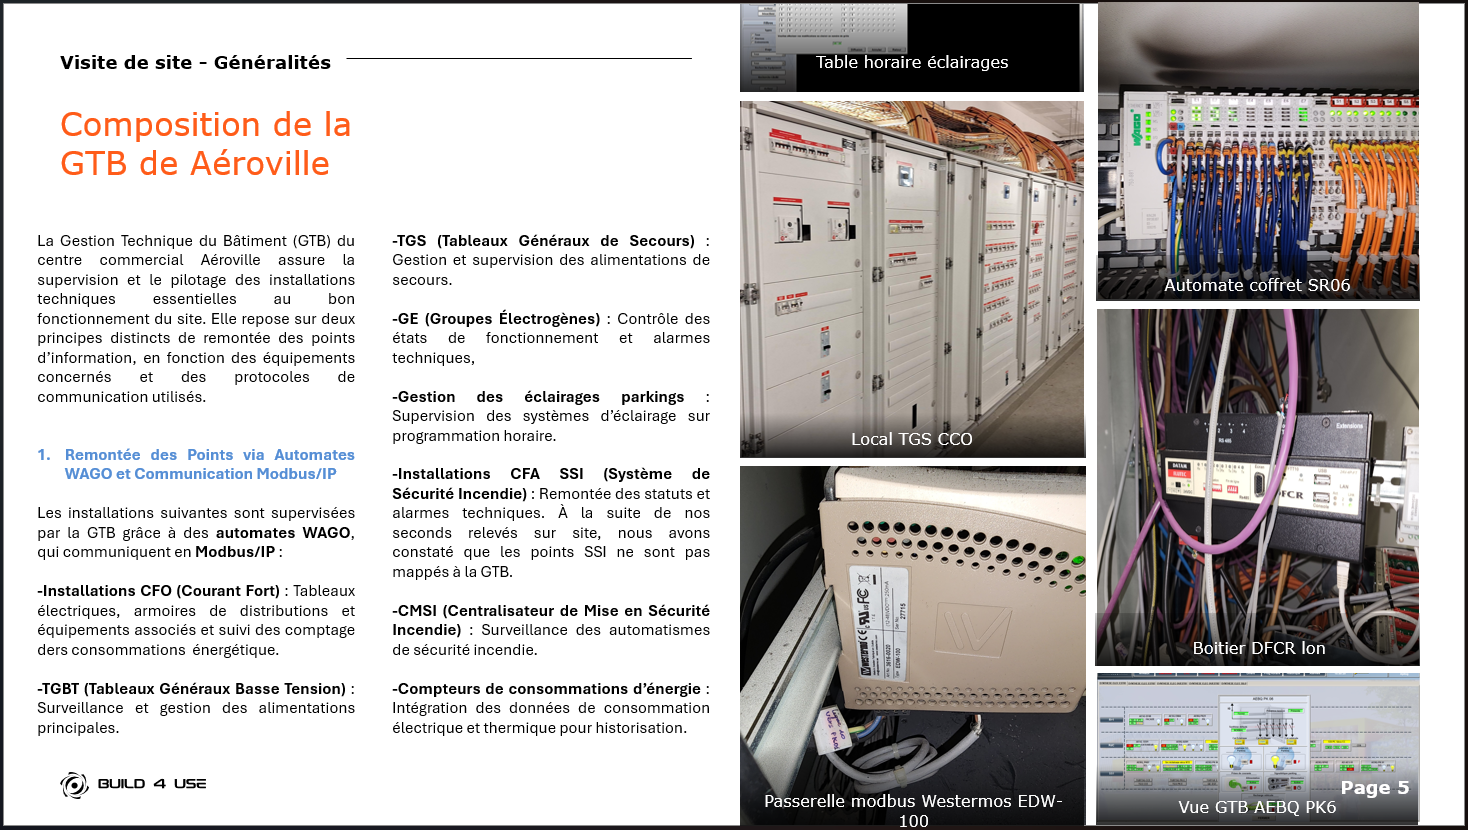
\includegraphics[width=\textwidth]{exemple.png}
    \caption{Slide de rapport d'audit AMO}
    \label{dash}
\end{figure}

\begin{figure}[h]
    \centering
    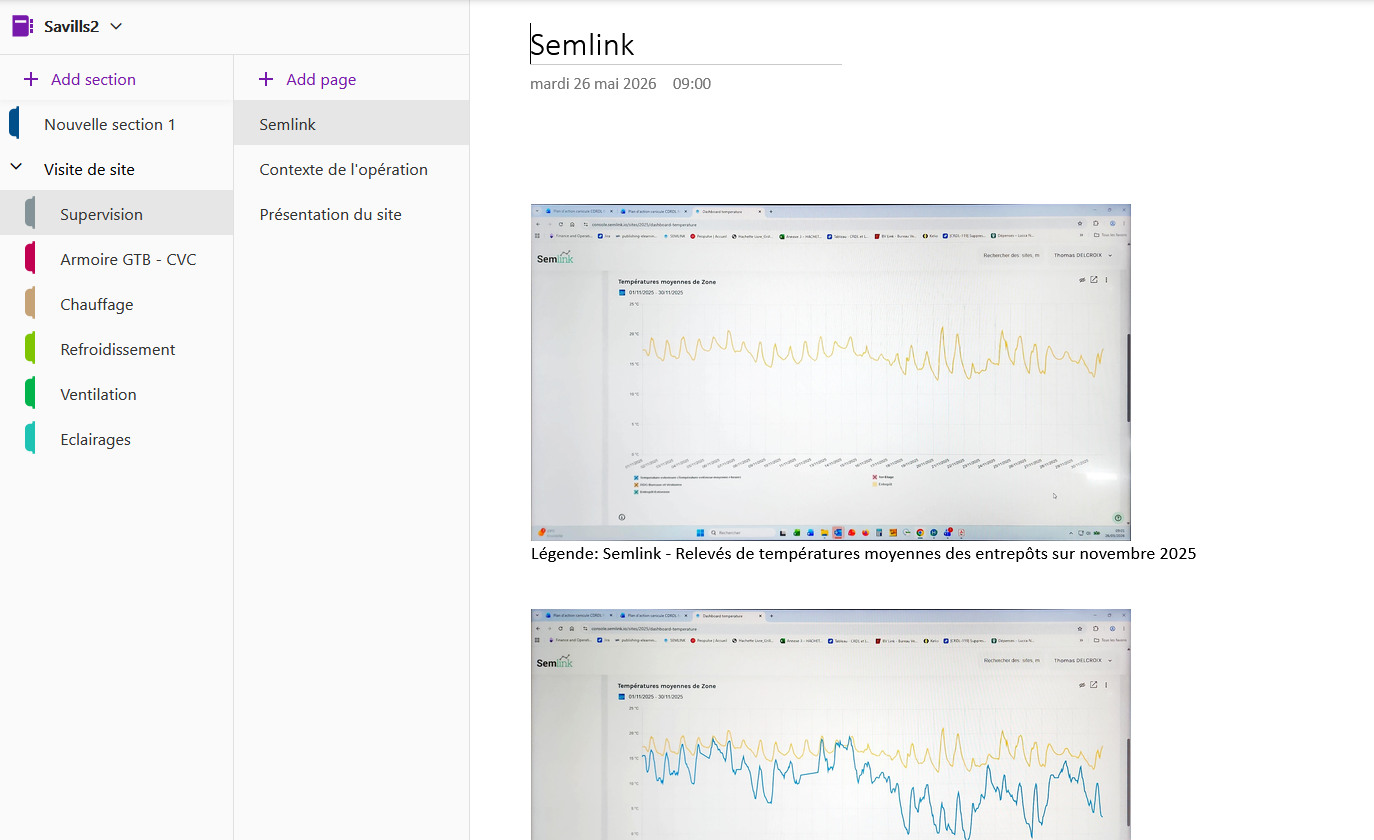
\includegraphics[width=\textwidth]{onenote.png}
    \caption{Relevé OneNote organisé}
    \label{dash}
\end{figure}

\begin{figure}[h]
    \centering
    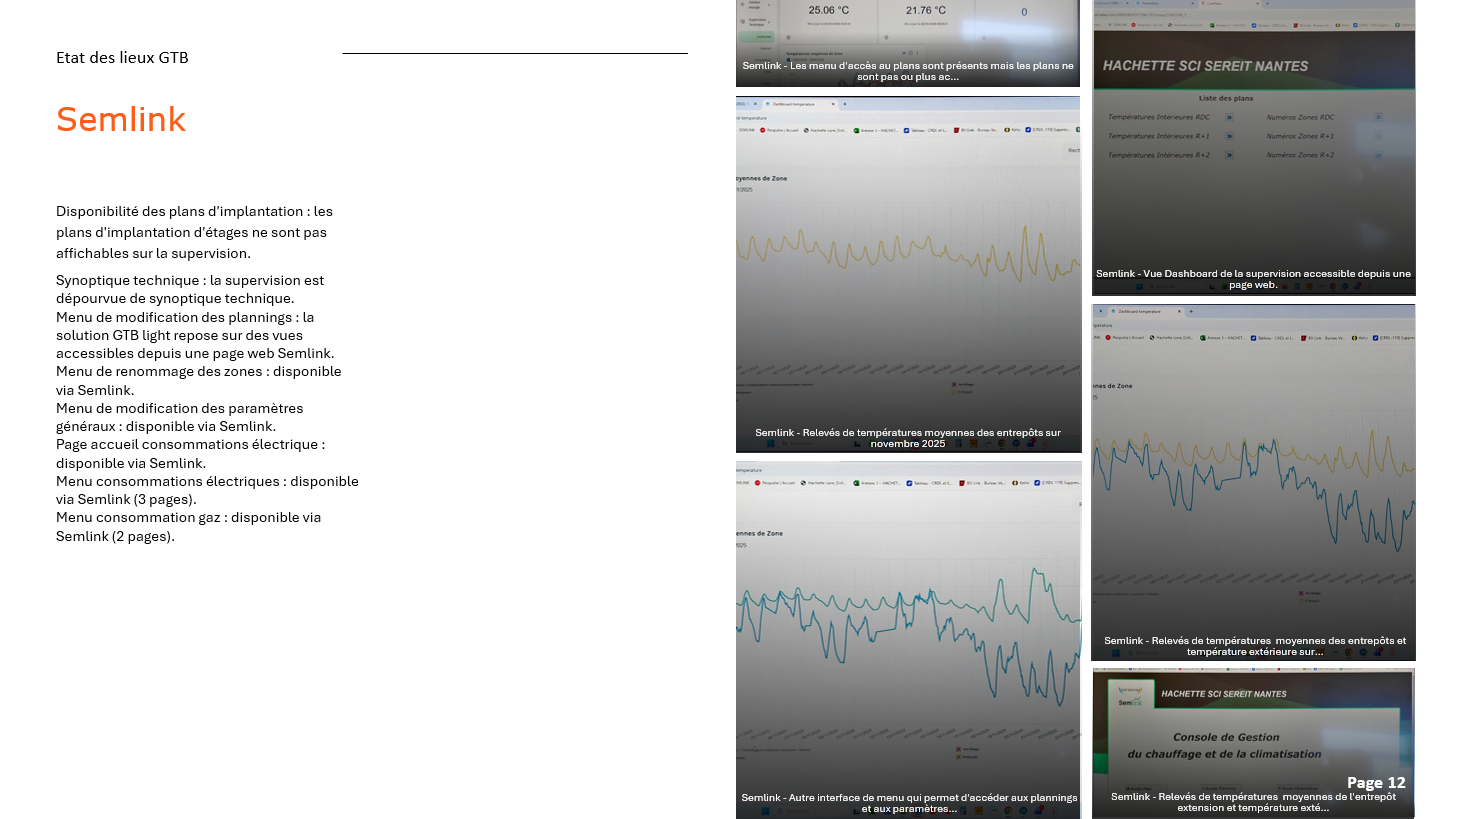
\includegraphics[width=\textwidth]{rapport.png}
    \caption{Slide de rapport d'audit généré}
    \label{dash}
\end{figure}

\begin{figure}[h]
    \centering
    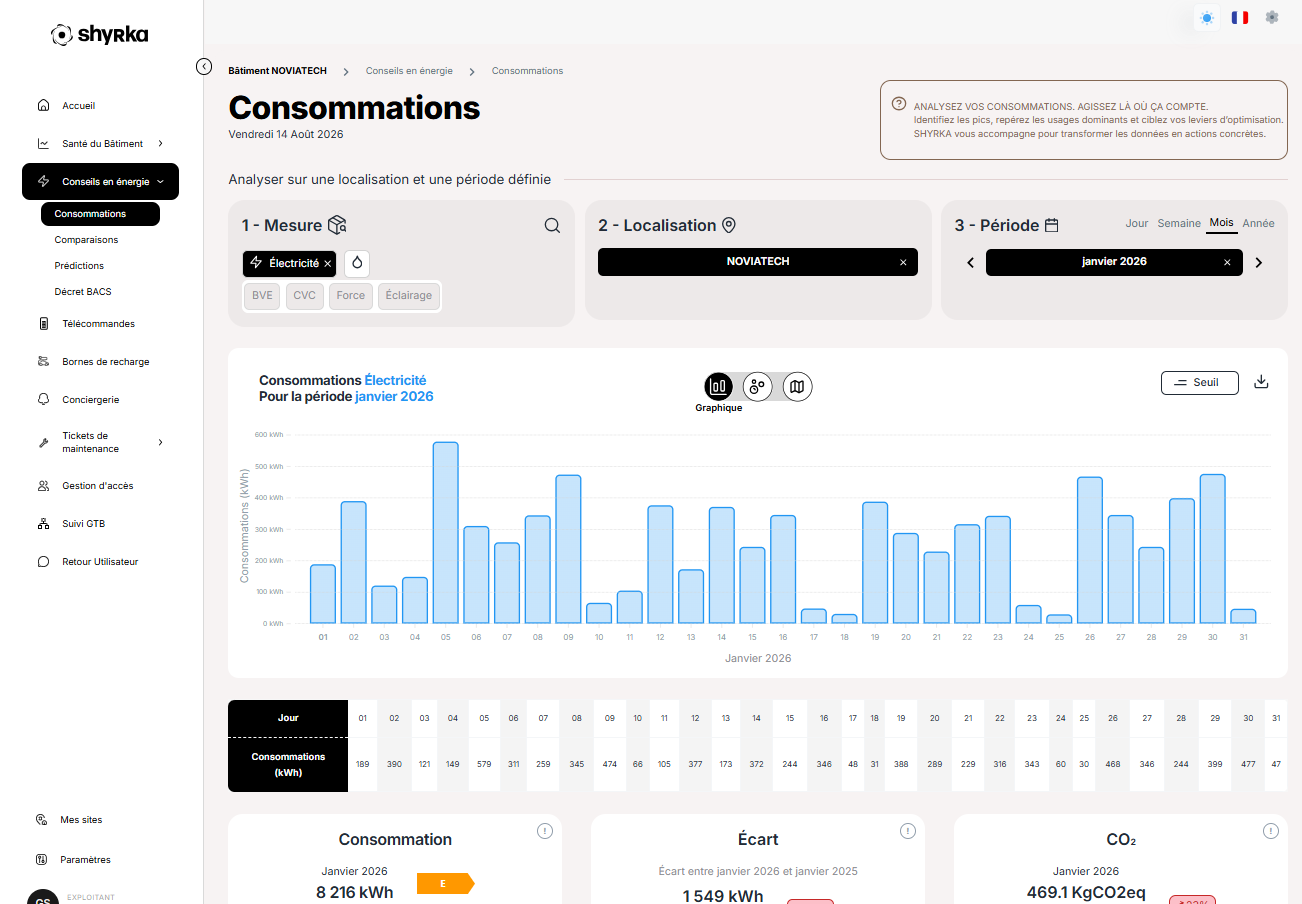
\includegraphics[width=\textwidth]{shyrka.png}
    \caption{Suivi des consommations via Shyrka}
    \label{dash}
\end{figure}

\begin{figure}[h]
    \centering
    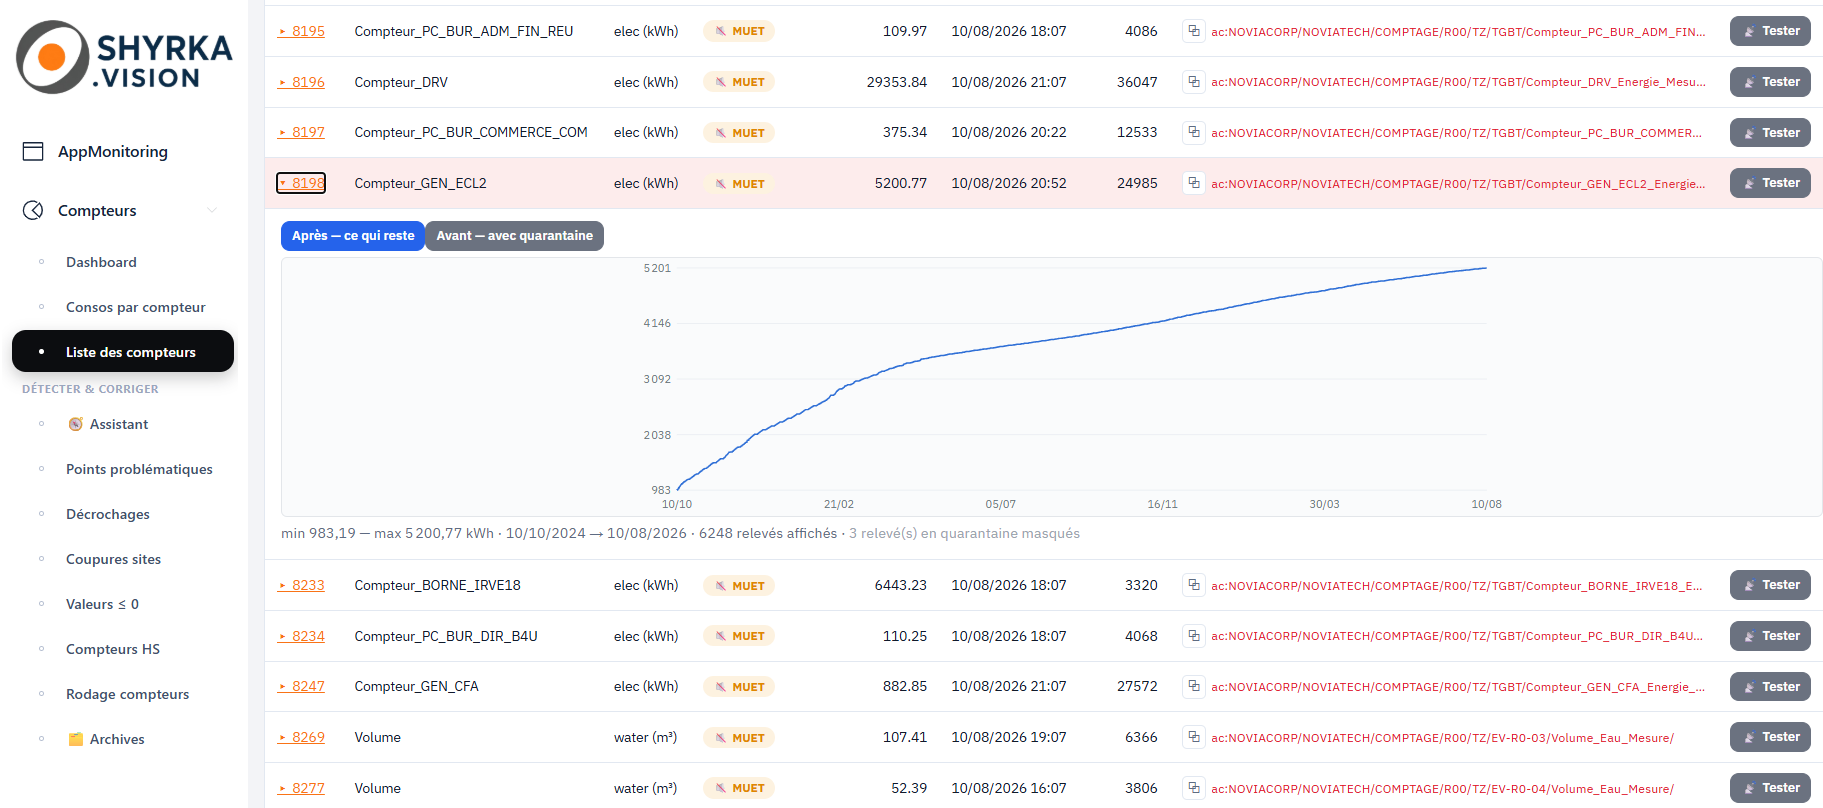
\includegraphics[width=\textwidth]{nettoyage.png}
    \caption{Nettoyage des historiques et compteurs via Shyrka Vision}
    \label{dash}
\end{figure}

\begin{figure}[h]
    \centering
    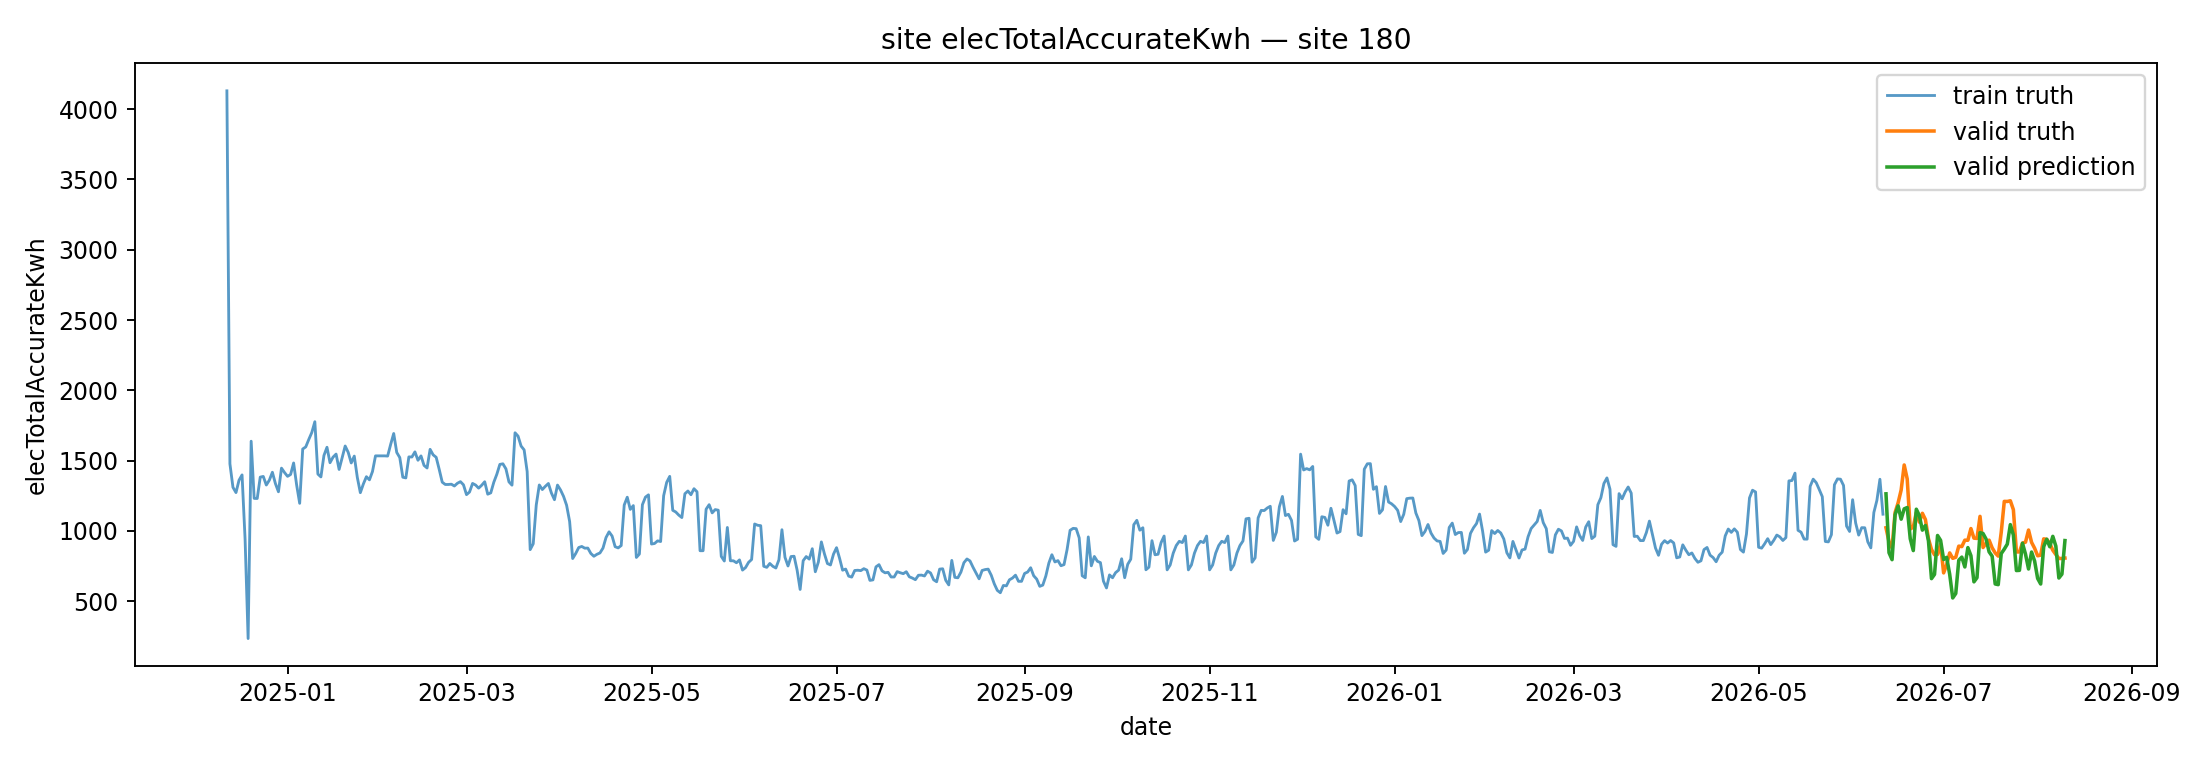
\includegraphics[width=\textwidth]{ts_site180_elecTotalAccurateKwh_train_valid.png}
    \caption{Courbe de consommation électrique}
    \label{dash}
\end{figure}

\begin{figure}[h]
    \centering
    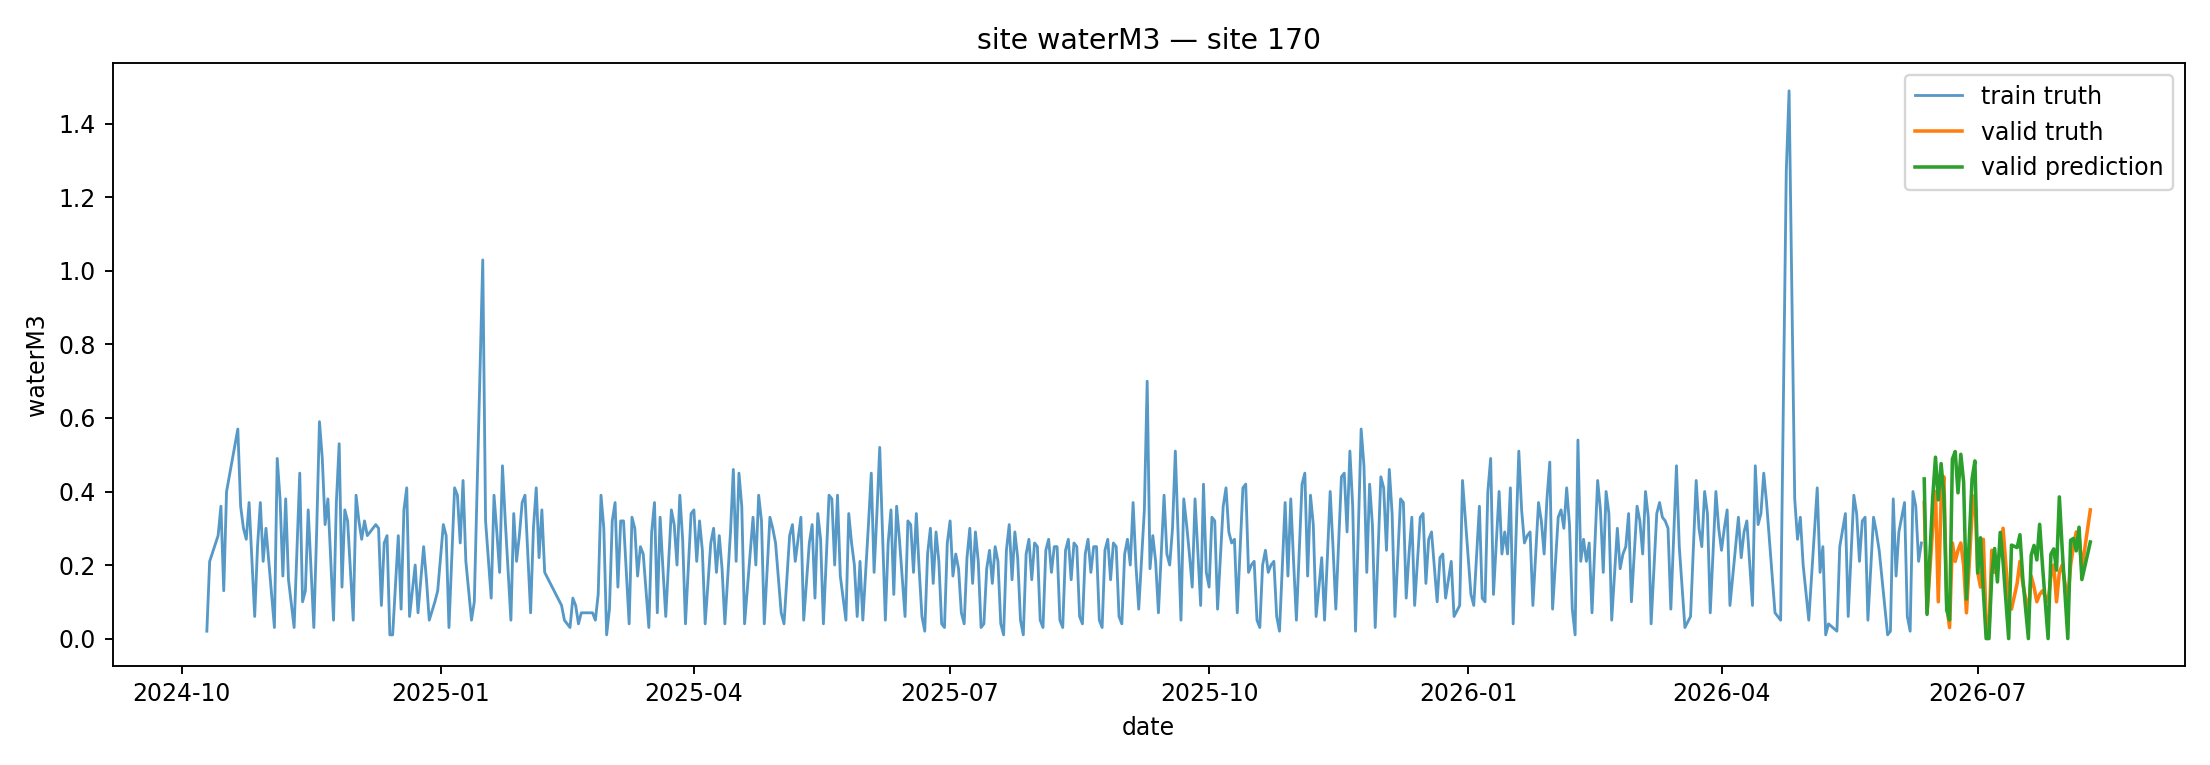
\includegraphics[width=\textwidth]{ts_site170_waterM3_train_valid.png}
    \caption{Courbe de consommation d'eau}
    \label{dash}
\end{figure}

\begin{figure}[h]
    \centering
    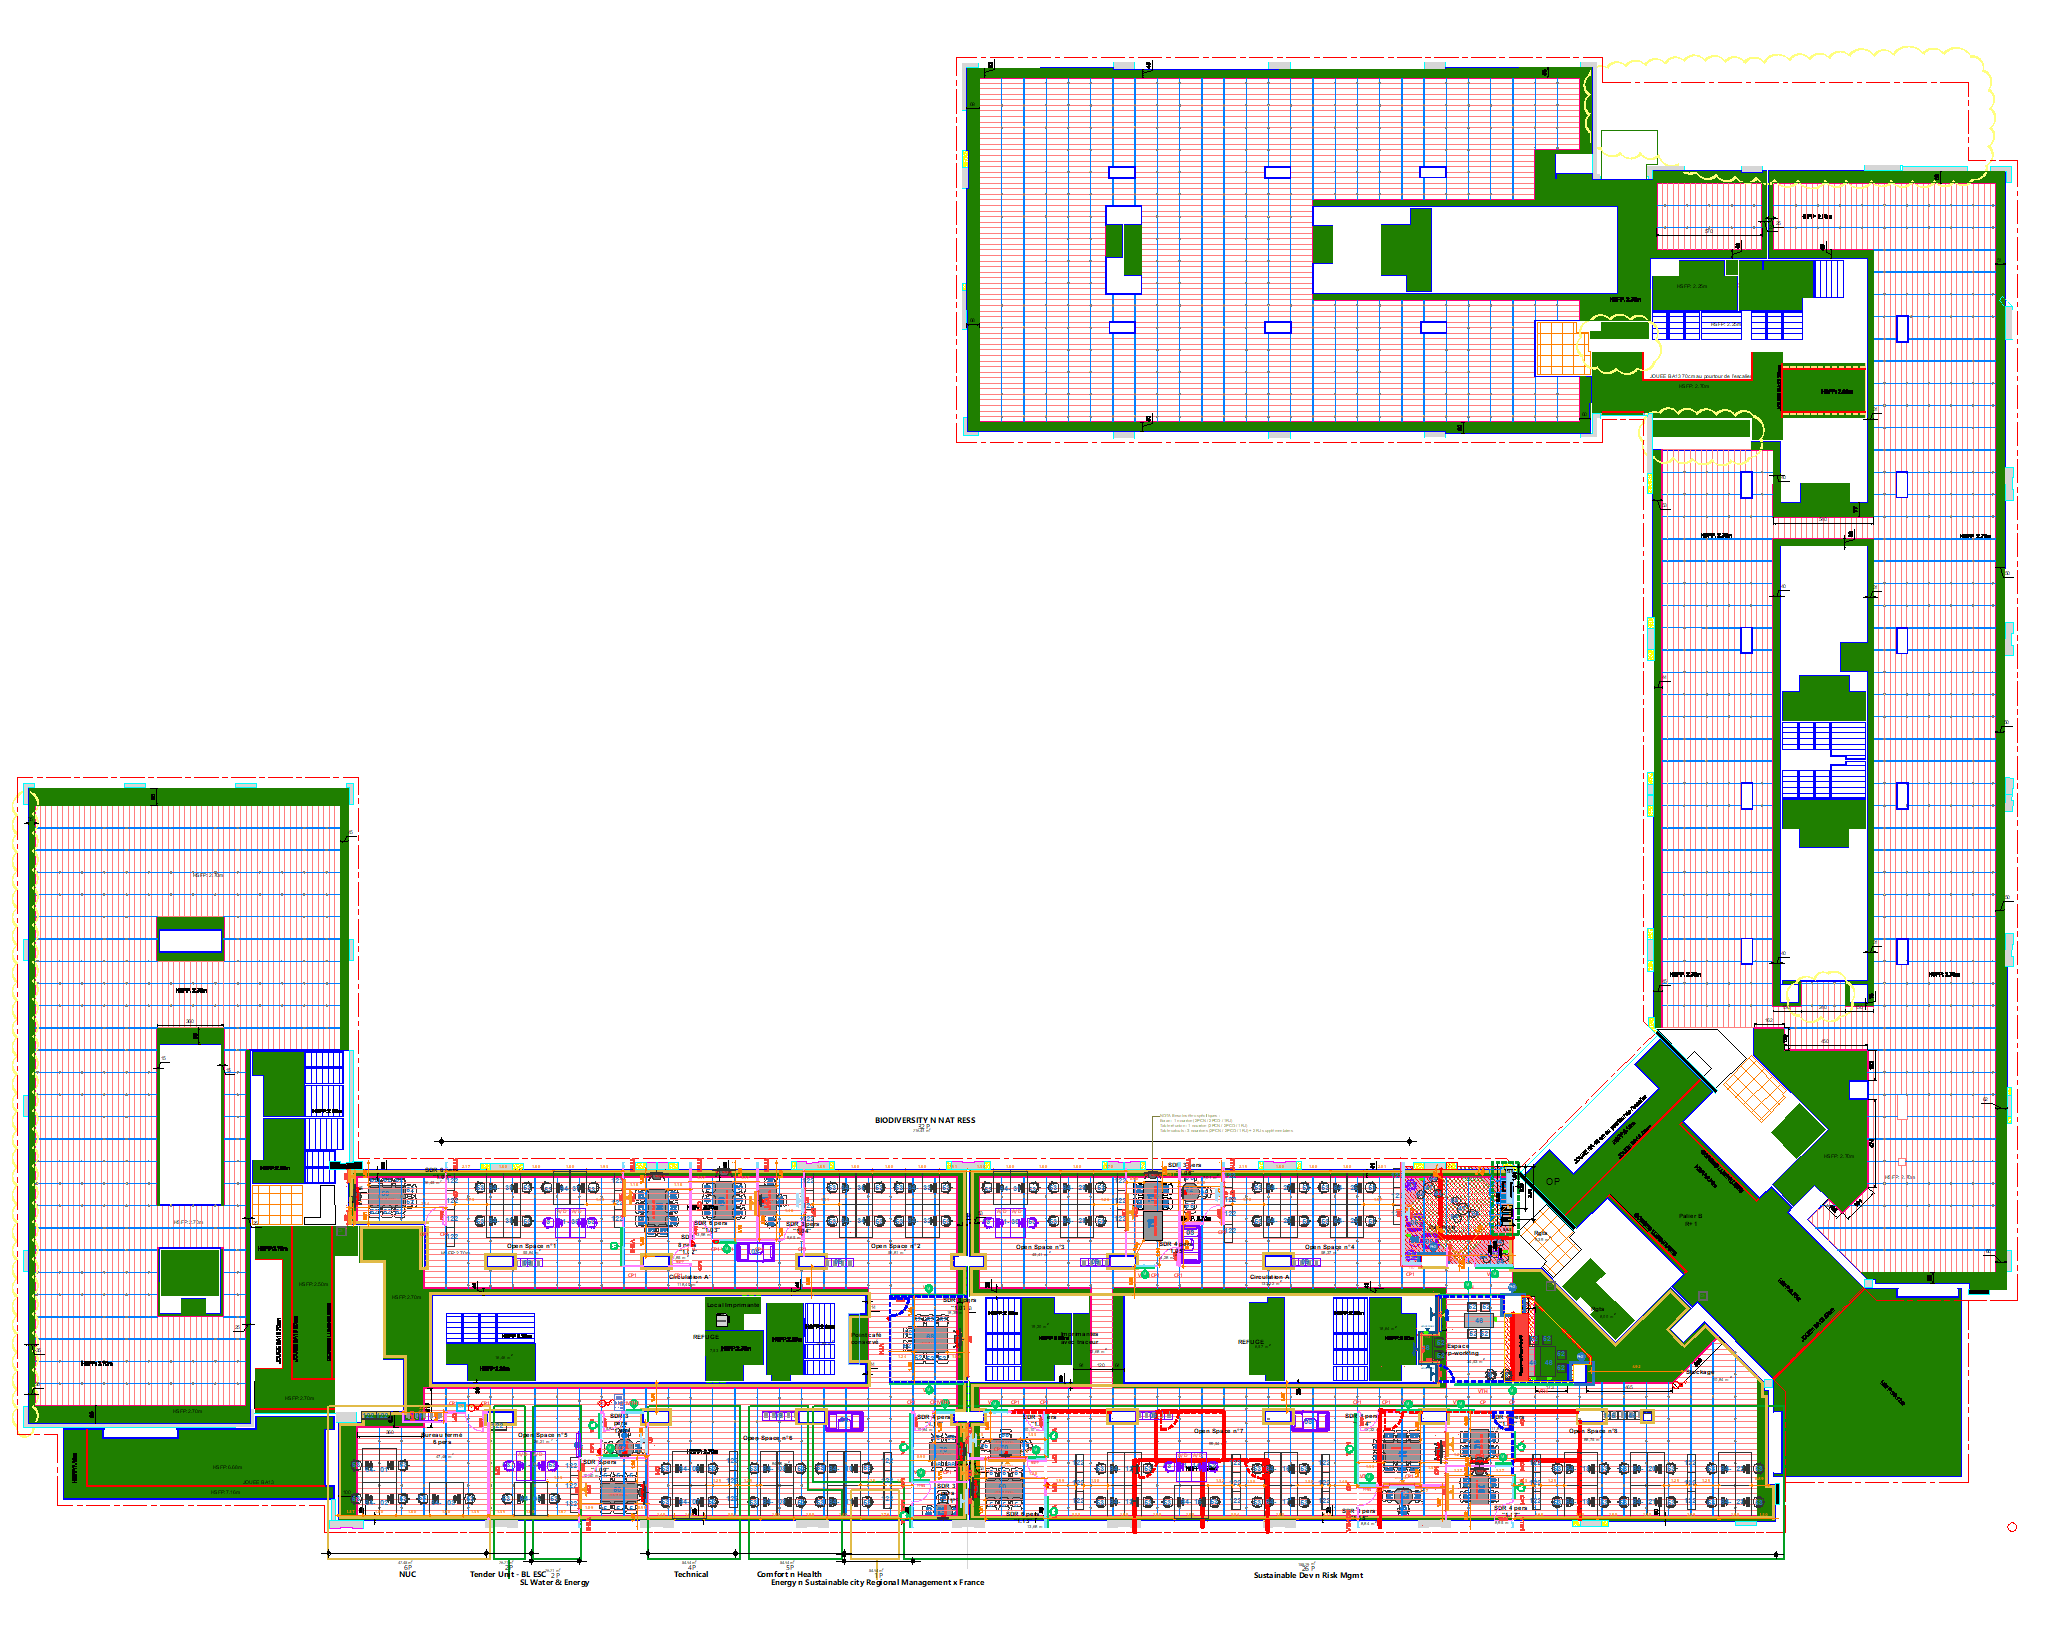
\includegraphics[width=\textwidth]{sample.Model.png}
    \caption{Plan AutoCAD}
    \label{dash}
\end{figure}

\begin{figure}[h]
    \centering
    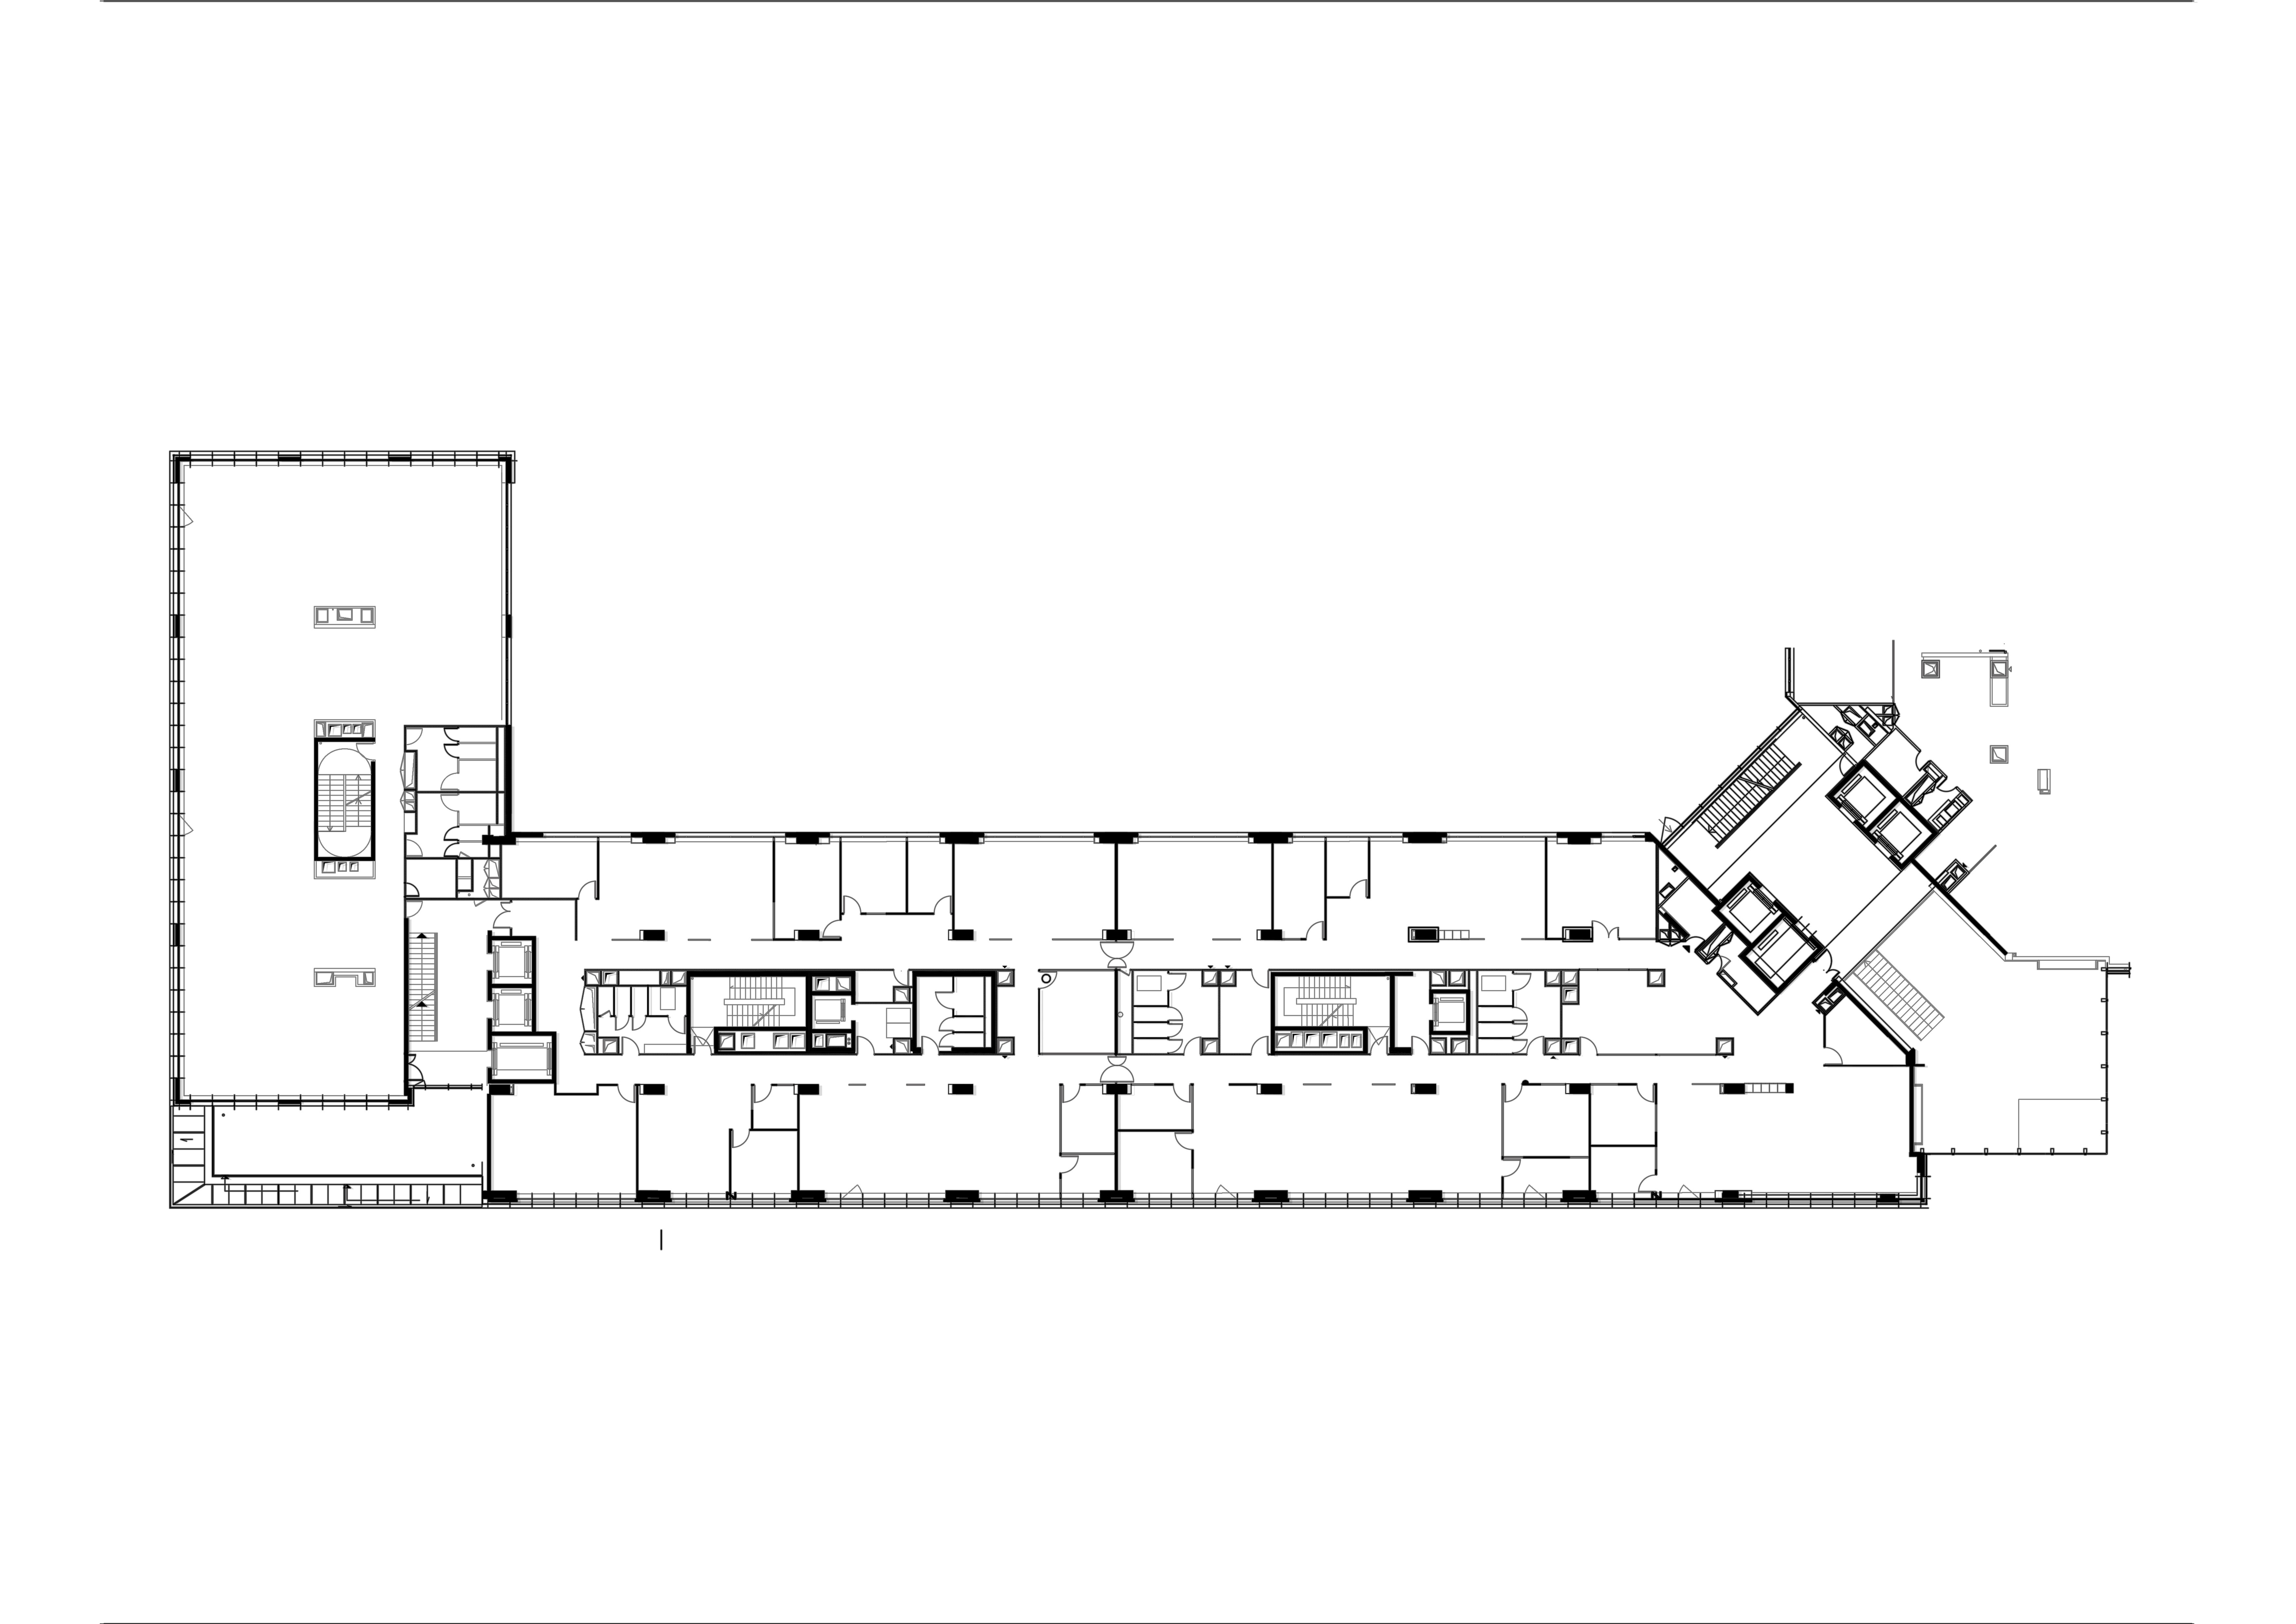
\includegraphics[width=\textwidth]{EGIS_Guyancourt_R+1_DET_20260306-INDICE-2-Model.jpg}
    \caption{Plan nettoyé via un contractuel}
    \label{dash}
\end{figure}

\begin{figure}[h]
    \centering
    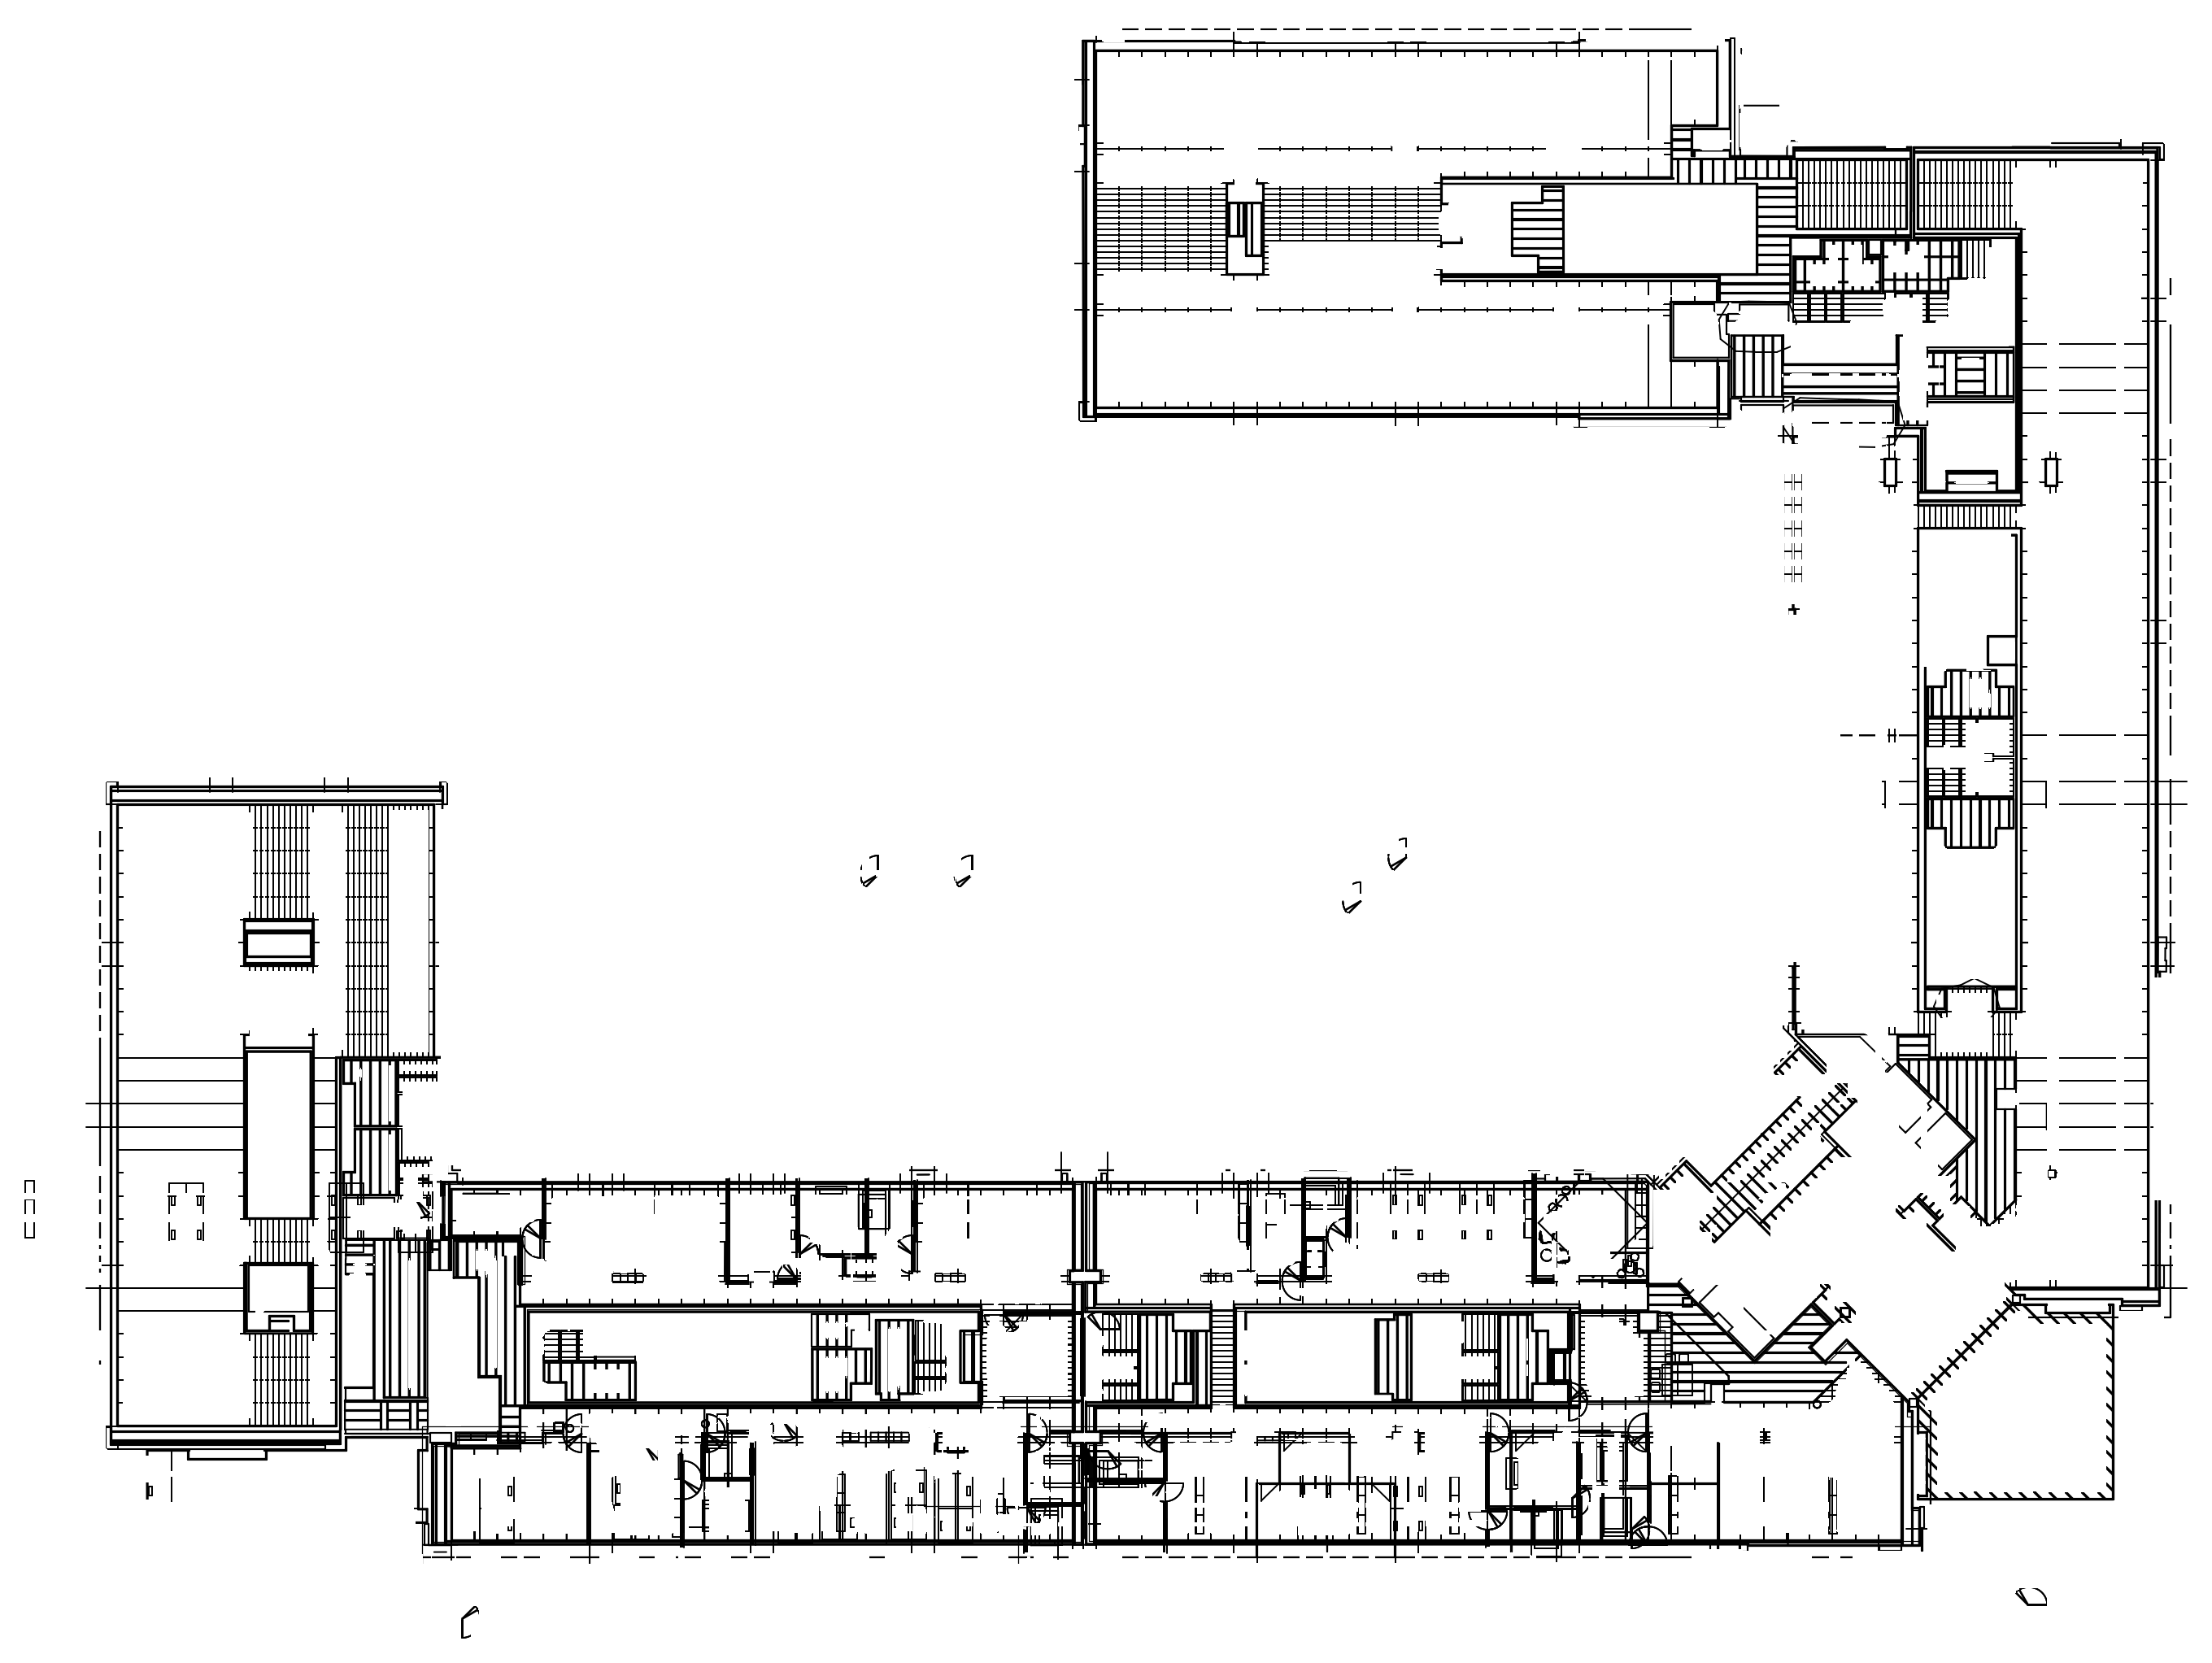
\includegraphics[width=\textwidth]{rendered_clean_v12_mesh_2d.png}
    \caption{Plan nettoyé par l'algorithme}
    \label{dash}
\end{figure}

\end{document}
